\documentclass[spanish]{udpreport}
\usepackage[utf8]{inputenc}
\usepackage[spanish]{babel}

% Podemos establecer el logo de alguna entidad o dejar el de la UDP (defecto)
%\setlogo{EITFI}

\title{Informe de redes de datos 7\\
"IETF:Protocolo de transferencia HTTP/2"\\}
\author{Alumno: Camilo Araya, Jose Undurraga, Boris Contreras
\\Profesor: Nicolás Hidalgo\\Ayudante: Martín Griño}
\date{\today}



\begin{document}
\maketitle

\chapter*{Resumen} 
\addcontentsline{toc}{section}{Resumen} 
\markboth{RESUMEN}{RESUMEN} 
Este es una documentación de normas de internet, generado gracias al consenso de la comunidad IETF. El documento citado para nuestro laboratorio fue aprobado por la comunidad publica y por el grupo de directivos de ingeniería de internet (IESG).El tema  que se abordara es el uso del protocolo HTTP/2 en el uso de las redes de datos. 
Esta especificación describe una expresión optimizada de la semántica del protocolo  de transferencia  de hipertexto HTTP, la cual es llamada HTTP versión 2 o “HTTP/2”. 
\\[0.2cm]
Este protocolo permite un uso más eficiente de los recursos de la red, además de entregar un resultado admisible de reducida latencia ocasionada por la compresión del campo HEADER  del HTTP, lo cual ocasiona múltiples intercambios simultáneos en la misma conexión.

\tableofcontents
\chapter{Introducción}
HTTP es el protocolo de transferencia de texto más exitoso, sin embargo la forma en que el protocolo HTTP/1.0 como HTTP/1.1 usa el transporte de texto tiene generalmente efectos negativos  en el rendimiento de las aplicaciones actuales.
\\[0.2cm]
En la actualidad el trafico de las redes se transformo en un tema de gran prioridad dado que su aumento se refleja de manera exponencial a medida que pasan los años, por lo que buscar formas de hacer que las redes trabajen de manera eficiente es el desafió de todos los profesionales que están inmerso en este medio.
\chapter{Preguntas a sus problemáticas}
\section{¿Por qué HTTP/1.0  y HTPP/1.1 produce efectos negativos?}
HTTP/1.0-> Solo una solicitud predomina en una conexión (TCP) en un lapso de tiempo determinado.
\\[0.2cm]
HTTP/1.1-> Canalización de las solicitudes, pero esto solo atiende las concurrencias de las solicitudes de forma parcial, por lo que aún sufren bloqueos de línea.
\\[0.2cm]
Por lo tanto, cuando los clientes realizan muchas solicitudes estos realizan conexiones múltiples en un servidor, de esta forma logran la concurrencia generando como resultado reducir las latencias. Además como los encabezados de campo HTTP tienden por lo general a ser repetitivos, generan  tráficos de redes innecesarios que congestionan la conexión.
\section{¿Existe una solución a este problema?}
HTTP/2 resuelve estos problemas realizando un mapeo optimizado de la semántica HTTP  a una conexión, mas específicamente permite la intercalación de los mensajes  de solicitud y respuesta en la misma conexión a través de la codificación eficiente de los encabezados de campo HTTP. Esto logra priorizar las solicitudes dando prioridad a los que logran completarse con mayor rapidez, esto genera una mejora en todo el rendimiento.
\\[0.2cm]
El protocolo HTTP/2 es más amigable para las redes dado que existe menos competencia entre los flujos y conexiones que tienen una mayor duración en su solicitud, esto conduce a una optimización en la utilización de la red disponible.
\chapter{Descripción general del protocolo HTTP/2}
1)	Propone un transporte óptimo para la semántica HTTP.
\\[0.2cm]
2)	Admite todas las características del protocolo HTTP/1.1 haciéndolas más eficientes que su predecesora.
\\[0.2cm]
3)	La unidad básica del protocolo HTTP/2 es una trama en la cual  cada tipo de marco tiene un propósito diferente:
\\[0.2cm]
HEADER Y DATA: Base de solicitud yy respuesta  de HTTP.
\\[0.2cm]
SETTING, WINDOWS-UPDATE Y PUSH-PROMISE:Son usados para soportar otras características del protocolo HTTP/2.
\\[0.2cm]
4)	Agrega un modo interactivo entre servidor y el cliente, mediante la impulsión de respuestas, esto a través del SERVER-PUSH, el cual envía (especulativamente) datos al cliente  de forma anticipada intercambiando parte del uso de la red, de esta forma se logra mapear el encabezado  de campo HTTP.
\\[0.2cm]
Esto genera una gran ventaja dado que permite que muchas solicitudes sean comprimidas en un paquete logrando la organización de la documentación.
\\
\begin{figure}[h]
    \centering
    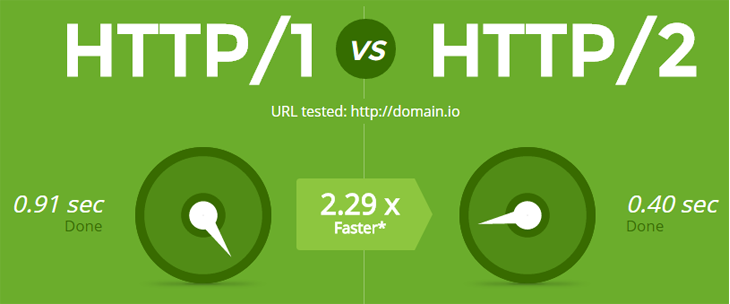
\includegraphics[scale=0.5]{images/http1-vs-http2.png}
    \caption{Comparación HTTP1 v/s HTTP2}
    \label{fig:my_label}
\end{figure}
\\
\chapter{Organización de la documentación}
\begin{figure}[h]
    \centering
    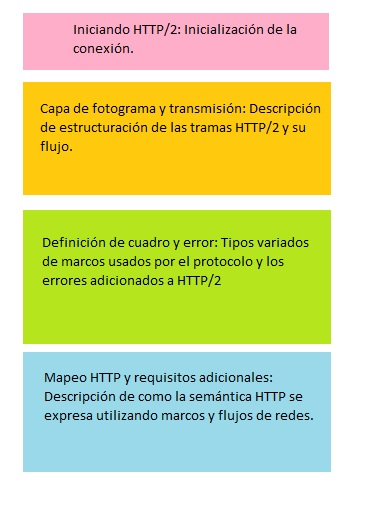
\includegraphics{images/qq1.jpg}
    \caption{Organización jerárquica}
    \label{fig:my_label}
\end{figure}
\\
\chapter{Conclusion}
Se puede deducir que el protocolo HTTP/2 permite un procesamiento más eficiente del tráfico de mensajes, mediante la utilización de estructuras  de mensajes binarios. 
\\
\begin{thebibliography}{0}
\bibitem{1}https://tools.ietf.org/wg/httpbis/draft-ietf-httpbis-http2/ \\ 
\end{thebibliography}
\listoffigures
\end{document}

